% Complete System Ontology — spans all three tiers
% Tier 1: Source-level extraction (high-level here — detailed schema in
%         knowledge-graph-ontology.tex)
% Tier 2: Aggregation
% Tier 3: Strategy + Execution Framework
%
% Compile with: pdflatex complete-ontology.tex
\documentclass[border=14pt]{standalone}

\usepackage[T1]{fontenc}
\usepackage[english]{babel}
\usepackage{lmodern}
\usepackage{amsmath}
\usepackage{amssymb}
\usepackage{xcolor}
\usepackage{tikz}
\usetikzlibrary{
    decorations.pathmorphing,
    decorations.pathreplacing,
    arrows.meta,
    positioning,
    calc,
    shapes.geometric,
    backgrounds,
    fit
}

%% ---------- Colour palette ----------
\definecolor{ink}        {HTML}{1F2433}
\definecolor{soft}       {HTML}{9CA3AF}
\definecolor{accent}     {HTML}{3A6E5B}
\definecolor{accentbg}   {HTML}{E4EFE9}

\definecolor{c1}{HTML}{4A6FA5}\definecolor{c1bg}{HTML}{EBF1F9}  % Topic
\definecolor{c2}{HTML}{C9883A}\definecolor{c2bg}{HTML}{FBF2DD}  % Author
\definecolor{c3}{HTML}{B85C92}\definecolor{c3bg}{HTML}{F8E8F0}  % Assumption
\definecolor{c4}{HTML}{4F8A6B}\definecolor{c4bg}{HTML}{E7F0EA}  % Theory
\definecolor{c5}{HTML}{C8553D}\definecolor{c5bg}{HTML}{FBEBE6}  % Conclusion
\definecolor{c6}{HTML}{5B6E8C}\definecolor{c6bg}{HTML}{ECEFF4}  % Methodology

\definecolor{ph1}{HTML}{4A6FA5}\definecolor{ph1bg}{HTML}{EBF1F9}  % Concept
\definecolor{ph2}{HTML}{C9883A}\definecolor{ph2bg}{HTML}{FBF2DD}  % Coaching/Impl
\definecolor{ph3}{HTML}{4F8A6B}\definecolor{ph3bg}{HTML}{E7F0EA}  % Integration

\definecolor{t1bg}   {HTML}{FBFCFE}
\definecolor{t2bg}   {HTML}{F8F6F2}
\definecolor{t3bg}   {HTML}{F4F7F5}
\definecolor{tborder}{HTML}{D5DAE3}

\begin{document}
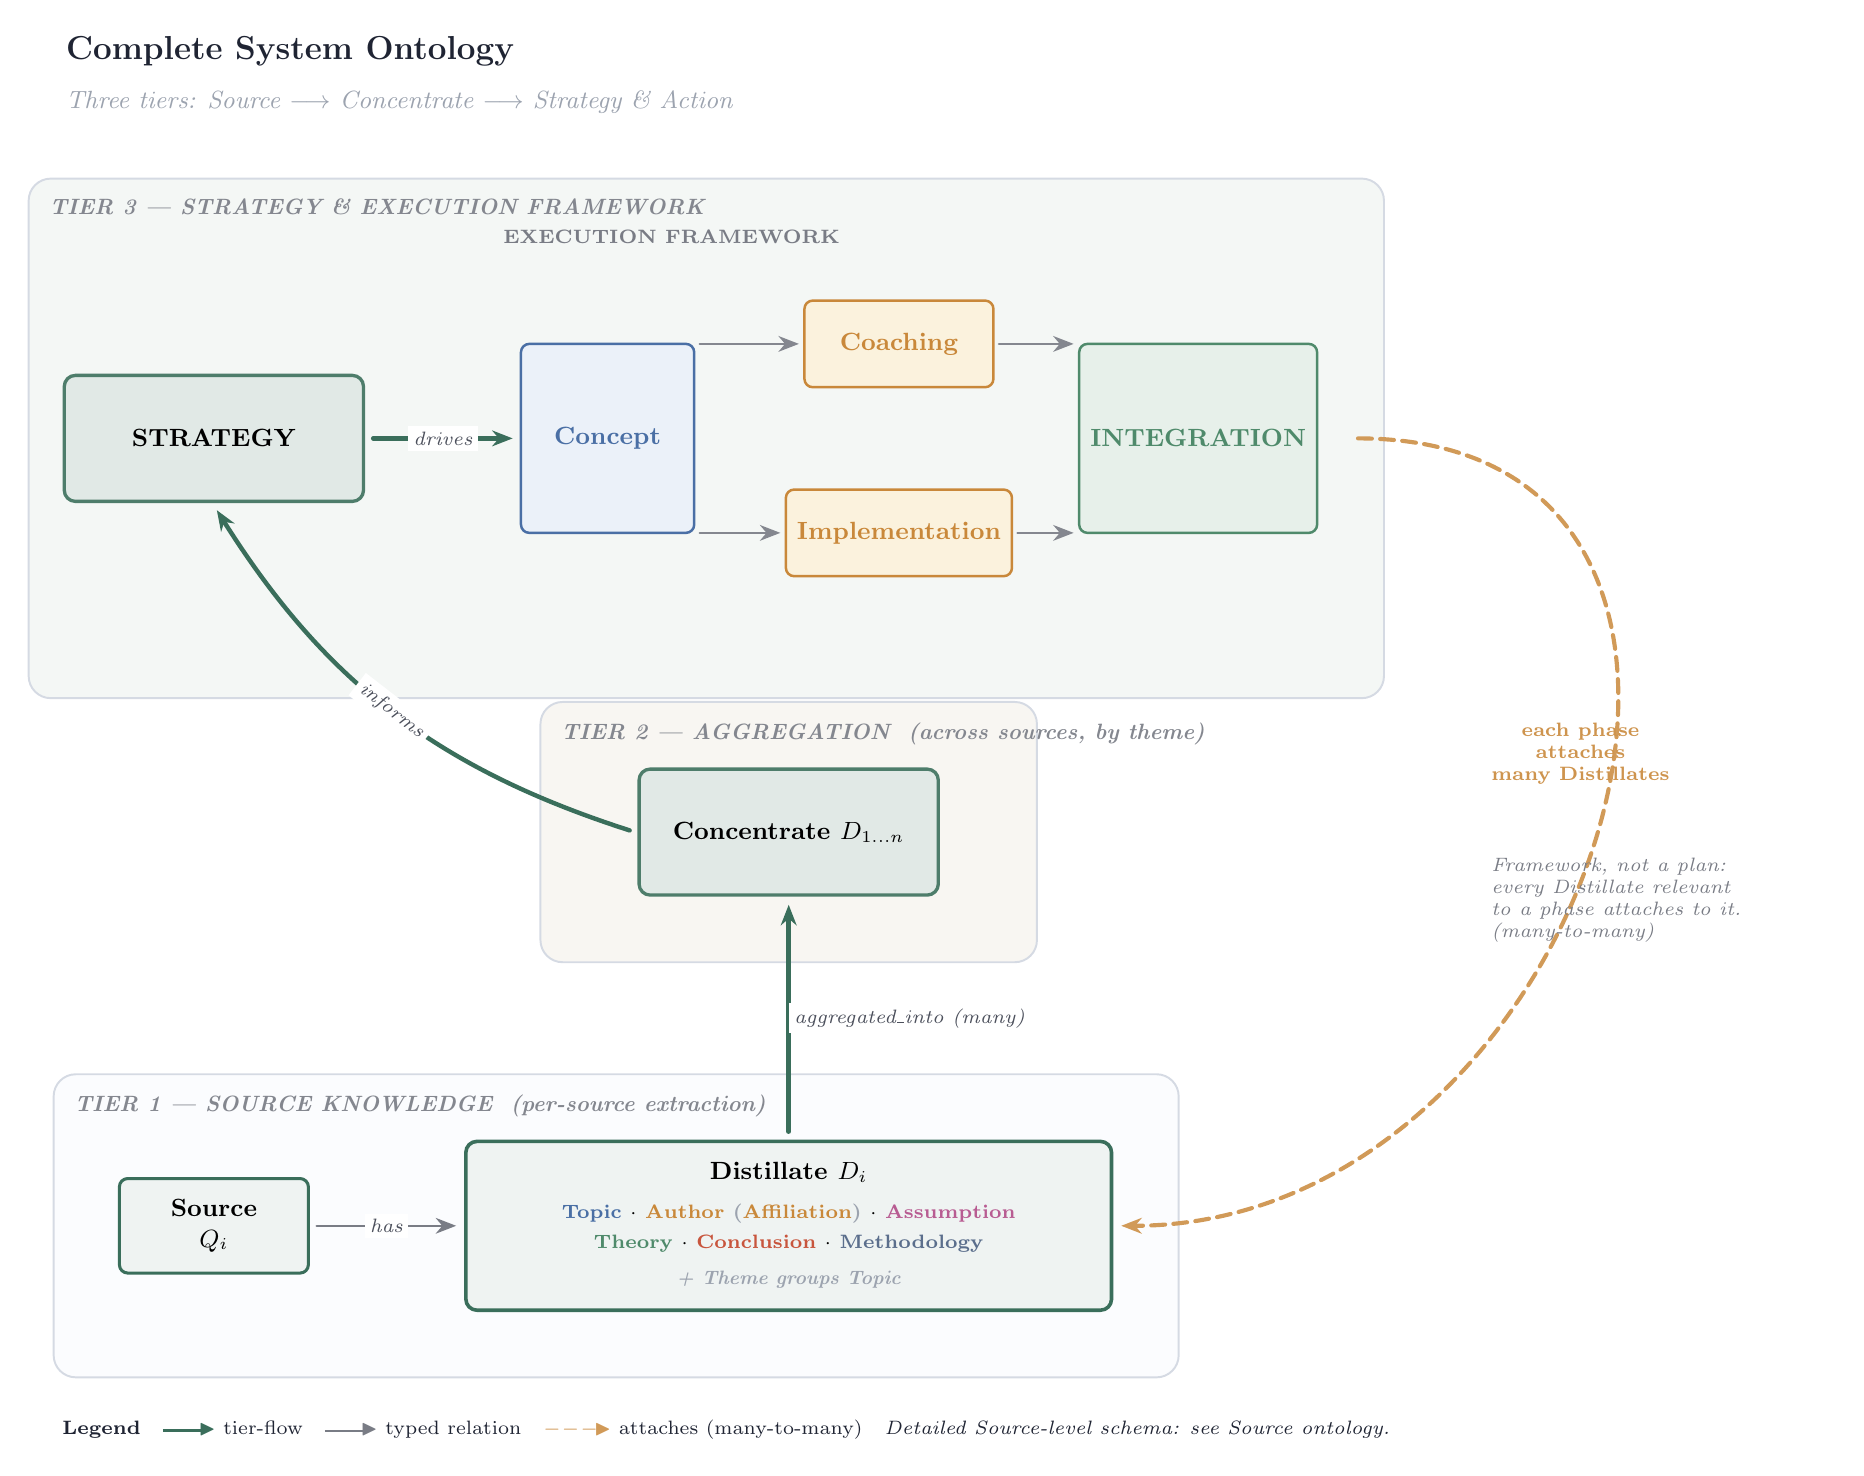
\begin{tikzpicture}[
    line cap=round, line join=round,
    >={Stealth[length=2.6mm, width=2.0mm]},
    entity/.style       = {rectangle, line width=0.9pt, rounded corners=3pt,
                           minimum width=24mm, minimum height=12mm,
                           font=\small\bfseries, align=center,
                           inner sep=4pt, outer sep=1pt},
    distentity/.style   = {rectangle, draw=accent, fill=accent!8,
                           line width=1.3pt, rounded corners=4pt,
                           align=center, inner sep=6pt, outer sep=1.5pt,
                           font=\small\bfseries},
    bigentity/.style    = {rectangle, line width=1.2pt, rounded corners=4pt,
                           minimum width=38mm, minimum height=16mm,
                           font=\small\bfseries, align=center,
                           inner sep=5pt, outer sep=1.5pt},
    pedge/.style        = {->, draw=ink!60, line width=0.9pt,
                           shorten >=2pt, shorten <=2pt},
    tieredge/.style     = {->, draw=accent, line width=1.6pt,
                           shorten >=2pt, shorten <=2pt},
    procflow/.style     = {->, draw=ink!55, line width=0.9pt,
                           shorten >=1pt, shorten <=1pt},
    attachedge/.style   = {->, draw=ph2!85, line width=1.5pt,
                           dash pattern=on 5pt off 3pt,
                           shorten >=2pt, shorten <=2pt},
    edgelabel/.style    = {font=\scriptsize\itshape, text=ink!80,
                           fill=white, inner sep=2pt, outer sep=0pt},
    tierlabel/.style    = {font=\footnotesize\bfseries\itshape, text=ink!55,
                           inner sep=2pt}
]

%% ============================================================
%% Title
%% ============================================================
\node[font=\large\bfseries, text=ink, anchor=south west]
    at (-7.5, 14.6) {Complete System Ontology};
\node[font=\small\itshape, text=soft, anchor=south west]
    at (-7.5, 14.0)
    {Three tiers: Source $\longrightarrow$ Concentrate $\longrightarrow$ Strategy \& Action};

%% ============================================================
%% TIER 1 — Source-level (compact; details in dedicated diagram)
%% ============================================================
\node[entity, fill=accent!8, draw=accent, line width=1.1pt]
    (Source) at (-5.5, 0) {Source\\$Q_i$};

\node[distentity, minimum width=82mm] (Dist) at (1.8, 0) {%
    \begin{tabular}{@{}c@{}}
        \bfseries Distillate $D_i$\\[3pt]
        {\scriptsize
            \textcolor{c1}{\bfseries Topic} $\cdot$
            \textcolor{c2}{\bfseries Author}
            {\color{soft}(\textcolor{c2}{Affiliation})} $\cdot$
            \textcolor{c3}{\bfseries Assumption}}\\
        {\scriptsize
            \textcolor{c4}{\bfseries Theory} $\cdot$
            \textcolor{c5}{\bfseries Conclusion} $\cdot$
            \textcolor{c6}{\bfseries Methodology}}\\[2pt]
        {\scriptsize\color{soft}\itshape + Theme groups Topic}
    \end{tabular}%
};

\draw[pedge] (Source) -- node[edgelabel] {has} (Dist);

% Tier 1 background
\begin{scope}[on background layer]
    \node[draw=tborder, fill=t1bg, rounded corners=8pt, line width=0.7pt,
          inner xsep=8mm, inner ysep=8mm,
          fit=(Source) (Dist)] (T1) {};
\end{scope}
\node[tierlabel, anchor=north west] at ($(T1.north west) + (2mm, -2mm)$)
    {TIER 1\ \textemdash\ SOURCE KNOWLEDGE \ (per-source extraction)};

%% ============================================================
%% TIER 2 — Aggregation
%% ============================================================
\node[bigentity, fill=accent!15, draw=accent!90]
    (Concentrate) at (1.8, 5.0) {Concentrate $D_{1\ldots n}$};

% Tier 2 background
\begin{scope}[on background layer]
    \node[draw=tborder, fill=t2bg, rounded corners=8pt, line width=0.7pt,
          inner xsep=12mm, inner ysep=8mm,
          fit=(Concentrate)] (T2) {};
\end{scope}
\node[tierlabel, anchor=north west] at ($(T2.north west) + (2mm, -2mm)$)
    {TIER 2\ \textemdash\ AGGREGATION \ (across sources, by theme)};

% Edge: Distillate aggregated into Concentrate
\draw[tieredge] (Dist.north) -- node[edgelabel, right]
    {aggregated\_into (many)} (Concentrate.south);

%% ============================================================
%% TIER 3 — Strategy + Execution Framework
%% ============================================================
\node[bigentity, fill=accent!15, draw=accent!90] (Strategy) at (-5.5, 10.0) {STRATEGY};

\node[entity, fill=ph1bg, draw=ph1, text=ph1,
      minimum width=22mm, minimum height=24mm]
    (Concept) at (-0.5, 10.0) {Concept};
\node[entity, fill=ph2bg, draw=ph2, text=ph2,
      minimum width=24mm, minimum height=11mm]
    (Coaching) at (3.2, 11.2) {Coaching};
\node[entity, fill=ph2bg, draw=ph2, text=ph2,
      minimum width=24mm, minimum height=11mm]
    (Impl) at (3.2,  8.8) {Implementation};
\node[entity, fill=ph3bg, draw=ph3, text=ph3,
      minimum width=22mm, minimum height=24mm]
    (Integ) at (7.0, 10.0) {INTEGRATION};

\draw[procflow] (Concept.east |- Coaching.west) -- (Coaching.west);
\draw[procflow] (Concept.east |- Impl.west)     -- (Impl.west);
\draw[procflow] (Coaching.east) -- (Integ.west |- Coaching.east);
\draw[procflow] (Impl.east)     -- (Integ.west |- Impl.east);

% Framework container
\begin{scope}[on background layer]
    \node[draw=ink!25, fill=white, rounded corners=5pt, line width=0.8pt,
          inner xsep=4mm, inner ysep=5mm,
          fit=(Concept) (Coaching) (Impl) (Integ)] (Framework) {};
\end{scope}
\node[font=\scriptsize\bfseries, text=ink!60, anchor=south west]
    at ($(Framework.north west) + (1mm, 0.5mm)$) {EXECUTION FRAMEWORK};

% Strategy/Concentrate connections
\draw[tieredge] (Concentrate.west) to[bend left=20]
    node[edgelabel, sloped, pos=0.5] {informs} (Strategy.south);
\draw[tieredge] (Strategy.east) -- node[edgelabel] {drives} (Concept.west);

% Tier 3 background
\begin{scope}[on background layer]
    \node[draw=tborder, fill=t3bg, rounded corners=8pt, line width=0.7pt,
          inner xsep=4mm, inner ysep=10mm,
          fit=(Strategy) (Framework)] (T3) {};
\end{scope}
\node[tierlabel, anchor=north west] at ($(T3.north west) + (2mm, -2mm)$)
    {TIER 3\ \textemdash\ STRATEGY \& EXECUTION FRAMEWORK};

%% ============================================================
%% Cross-tier ATTACHES (the key new insight)
%% ============================================================
% Wide arc on the right: Framework → Distillate (many-to-many attachment)
\draw[attachedge]
    (Framework.east) to[out=0, in=0, looseness=1.5]
    (Dist.east);

\node[font=\scriptsize\bfseries, text=ph2!90, align=center, anchor=west]
    at (10.6, 6.0)
    {each phase\\\textbf{attaches}\\many Distillates};

\node[font=\scriptsize\itshape, text=ink!60, align=left, anchor=north west]
    at (10.6, 4.8)
    {\textit{Framework, not a plan:}\\
     every Distillate relevant\\
     to a phase attaches to it.\\
     (many-to-many)};

%% ============================================================
%% Legend
%% ============================================================
\node[anchor=north west, font=\scriptsize, text=ink]
    at ($(T1.south west) + (0, -4mm)$)
    {\textbf{Legend}\quad
     \textcolor{accent}{\rule[0.3ex]{5mm}{1pt}\!$\blacktriangleright$}~tier-flow\quad
     \textcolor{ink!60}{\rule[0.3ex]{5mm}{0.6pt}\!$\blacktriangleright$}~typed relation\quad
     \textcolor{ph2!85}{$-\!-\!-$\!$\blacktriangleright$}~attaches (many-to-many)\quad
     \emph{Detailed Source-level schema: see Source ontology.}};

\end{tikzpicture}
\end{document}
